\documentclass[
	12pt,
	a4paper,
	BCOR10mm,
	%chapterprefix,
	DIV14,
	listof=totoc,
	bibliography=totoc,
	headsepline
]{scrreprt}

\usepackage[T1]{fontenc}
\usepackage[utf8]{inputenc}
\usepackage[ngerman]{babel}

\usepackage{lmodern}

\usepackage[footnote]{acronym}
\usepackage[page,toc]{appendix}
\usepackage{fancyhdr}
\usepackage{float}
\usepackage{graphicx}
\usepackage[pdfborder={0 0 0}]{hyperref}
\usepackage[htt]{hyphenat}
\usepackage{listings}
\usepackage{lscape}
\usepackage{microtype}
\usepackage{nicefrac}
\usepackage{subfig}
\usepackage{textcomp}
\usepackage[subfigure,titles]{tocloft}
\usepackage{units}
\usepackage{pgf}
\usepackage{amsmath}
\usepackage{placeins}
\usepackage{titletoc}
\usepackage{todonotes}

\lstset{
	basicstyle=\ttfamily,
	frame=single,
	numbers=left,
	language=C,
	breaklines=true,
	breakatwhitespace=true,
	postbreak=\hbox{$\hookrightarrow$ },
	showstringspaces=false,
	tabsize=4
}

\renewcommand*{\lstlistlistingname}{Listing catalog}

\renewcommand*{\appendixname}{Appendix}
\renewcommand*{\appendixtocname}{Appendices}
\renewcommand*{\appendixpagename}{Appendices}


\begin{document}

\begin{titlepage}
	\begin{center}
		{\titlefont\huge Arbeitstitel: Analyse Wissenschaftlicher Daten mit BigData Werkzeugen \par}

		\bigskip
		\bigskip

		{\titlefont\Large --- Exposé ---\par}

		\bigskip
		\bigskip

		{\large Arbeitsbereich Wissenschaftliches Rechnen\\
		Fachbereich Informatik\\
		Fakultät für Mathematik, Informatik und Naturwissenschaften\\
		Universität Hamburg\par}
	\end{center}

	\vfill

	{\large \begin{tabular}{ll}
		Vorgelegt von: & Arne Struck \\
		E-Mail-Adresse: 
			& \href{mailto:1struck@informatik.uni-hamburg.de}{1struck@informatik.uni-hamburg.de} \\ 
		%Matrikelnummer: & 1234567 \\
		Studiengang: & Bsc. Informatik \\
		\\
		Betreuer: & Julian Kunkel \\
		\\
		Hamburg, den 21. Juni 2015%\today
	\end{tabular}\par}
\end{titlepage}

\thispagestyle{empty}

\newpage\null\thispagestyle{empty}\newpage
\tableofcontents
\newpage\null\thispagestyle{empty}\newpage

\chapter{Einleitung}
\label{einleitung}
\section{Motivation}
Der Bereich des High Performance Computing ist seit Jahrzehnten ein wichtiges Forschungs- und Anwendungsgebiet der Informatik.
Oftmals befasst sich das High Performance Computing mit Fragen der Meteorologie, Klimatologie, theoretischen Physik und Biologie.
Die Lösungen dieser Fragen wird durch die Simulation von Modellen aus dem entsprechenden Bereich und die Analyse von gemessenen und berechneten Daten approximiert. \\
Dies sind meist sehr rechenintensive Tätigkeiten, daher sind extrem leistungsstarke Rechner von Nöten.
Heutzutage werden zu diesem Zweck meistens Cluster, also verteilte Rechensysteme eingesetzt.
Bei der Realisierung der oben erwähnten Tätigkeiten auf verteilten Systemen ist die Frage der Parallelisierung von Berechnungen eine entscheidende. 
Im High Performance Computing Bereich wird dies seit Jahrzehnten großteilig durch Message Passing Interface MPI (beispielsweise implementiert durch Open MPI) erreicht \cite{HLR}. \\
Durch das Aufkommen des Internets als Massenmedium in den letzten beiden Jahrzehnten hat sich eine Ökonomie entwickelt, welche große Datenmengen managen und verarbeiten muss.
Auch diese Ökonomie, deren Geschäftsfeld allgemein als Big Data bezeichnet wird, setzt stark auf verteilte Systeme.

Allerdings wird hier nicht auf MPI für das Arbeiten auf verteilten Systemen gesetzt, sondern andere Lösungen für die Problematiken, welche verteilte Berechnungen mit sich bringen, bevorzugt.
Als Beispiel für Komplettlösungen wären spark und hadoop zu nennen, welche nicht auf dem MPI-Technologie Stack aufbauen. 
Allerdings existieren auch Werkzeuge, welche sich in die bisherigen Systeme leichter integrieren lassen, wie das Data Base Management System Rasdaman. \\
Diese Herangehensweisen versprechen leichtere Nutzbarkeit und Umsetzbarkeit durch Reduktion des durch die Parallelisierung bedingten Overheads im Programm, sowie höhere Flexibilität des Codes.
Analysen der Interessenlagen bezüglich der verschiedenen Herangehensweisen weisen auf einen Trend in Richtung der Lösungen der Big Data Unternehmen hin, wie in Abbildung \ref{fig:hpcdies1} und \ref{fig:hpcdies2} zu sehen. 
\begin{figure}[ht]
\centering
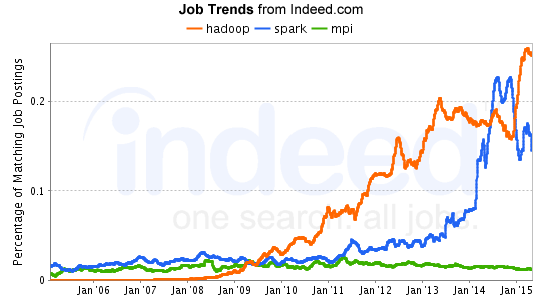
\includegraphics[scale=0.8]{./pics/jobgraph.png}
\caption{Jobangebote im betrachteten Bereich}
\label{fig:hpcdies1}
\end{figure}
\begin{figure}[ht]
\centering
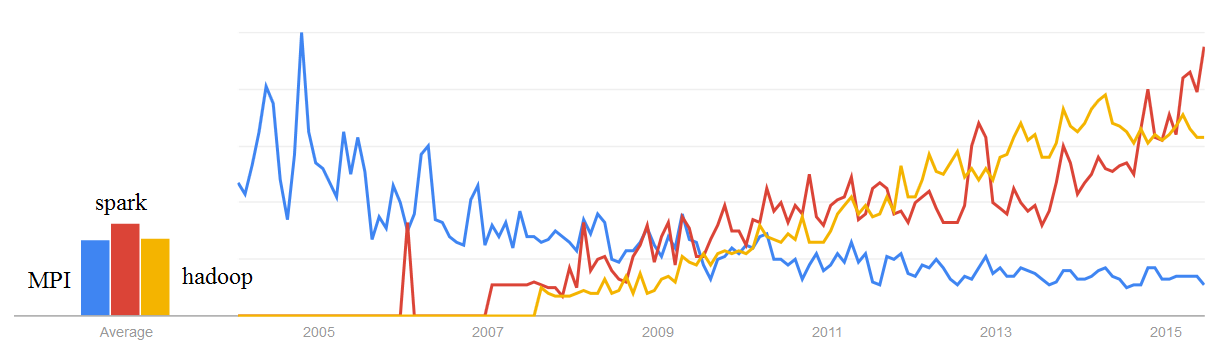
\includegraphics[width=1\textwidth, height=150px]{./pics/trends.png}
\caption{Google Trends: MPI, Spark, Hadoop}
\label{fig:hpcdies2}
\end{figure}
Die ''Big Data Unternehmen'' besitzen weiterhin das Potential High Performance Computing in Größenordnungen anzubieten, welche durchaus die der HPC Community übersteigen (erste Tendenzen in diese Richtung sind momentan zu beobachten \cite{HLR}). \\
Wegen der Verschiebung der Interessenlagen, der relativen Schwerfälligkeit MPIs und nicht zuletzt der Übermacht der Privatwirtschaft drängen sich für das klassische HPC die Frage auf, beziehungsweise ob die Lösungen aus der Big Data Ökonomie leistungstechnisch mit MPI konkurrieren können und somit eine zumindest partielle Alternative auch für die momentane High Performance Computing Community darstellen.\\
Die momentane Messungslage deutet darauf hin, dass die Werkzeuge aus der Big Data Industrie für die Berechnung von Simulationen nicht ausreicht \cite{HLR}.
Allerdings ist es möglich, dass ihre Leistungsfähigkeit für die Nachbereitung und Analysetätigkeiten im HPC-Bereich ausreichend ist. \\
\todo[inline]{hier kurze Beschreibung gestalten der Nachbereitung gestalten?}
\FloatBarrier

\section{Zielsetzung}
\label{ziel}
Diese Arbeit soll nun die zuvor erwähnte Eignung einiger ''Big Data'' Werkzeuge im Bezug auf die Nachbereitung wissenschaftlicher Daten analysieren.
Hierzu muss sowohl ein Vergleich untereinander, als auch zu den bisherigen Verfahrensweisen gezogen werden.
Für einen aussagekräftigen Vergleich für die Nutzbarkeit sind sowohl eine Bewertung des Bedienkomforts, als auch ein Vergleich der jeweiligen Einarbeitungszeiten und Nutzungszeiten.


\chapter{Problemstellung}
\label{Problemstellung}
Um das in \ref{ziel} definierte Ziel zu erreichen müssen viele Problematiken gelöst werden.
Da die Palette der in Frage kommenden Werkzeuge nahezu keine Grenzen kennt, muss eine Auswahl orientiert am begrenzten Zeitraum der Arbeit getroffen werden.
Da sowohl eine Einarbeitungszeit in die jeweiligen Werkzeuge, als auch eine Umsetzung für jedes Werkzeug von Nöten sind, aber auch eine gewisse Varianz von Nöten ist, wären 3 Werkzeuge eine naheliegende Wahl. 
Um die Integrierbarkeit in andere Systeme zu gewährleisten und die Einarbeitungszeit nicht durch das Aufsetzen ganzer Systeme zu beschränken, sollte die Wahl auf nicht Komplettlösungen eingeschränkt werden. \\
Ein weiteres Teilproblem der Eignungsbewertung stellt der Entwurf einheitlicher, geeigneter Testdaten dar.
Hierzu sollten die Daten sowohl eine ausreichende Größe besitzen, als auch aus dem High Performance Computing stammen. \\
Des weiteren muss eine Herangehensweise zur eigentlichen Eignungsanalyse gestaltet werden. 
Dieses Teilproblem gliedert sich in zwei Problemteile, zum einen die Definition der Bewertungskriterien, zum anderen Definitionen standardisierter Beispielfunktionalitäten und Herangehensweisen an die Messungen.

\todo[inline]{unsicher, ob im Sinne des Erfinders}


\chapter{Theoretischer Hintergrund}
\label{Theoretischer Hintergrund}
Im HPC-Bereich werden heutzutage große, berechnungsintensive Modelle berechnet. 
Im wissenschaftlichen Bereich heißt dies, dass es sich um Modelle komplexer Systeme handelt.
Ein Beispiel wäre hier ein Klimamodell, wobei Einzelheiten wie Wolkensysteme bis hin zu Verdunstungsmengen im Meer berechnet werden.
Dies ist nötig, da sich bei solchen Systemen, wie dem Klima alle Teilsysteme sich gegenseitig beeinflussen und das Einführen von nicht berechneten Einflüssen durch Konstanten oder das nicht beachten selbiger Einflüsse zu den Ungenauigkeiten der Berechnungen beiträgt. \\
Dies bedeutet, dass die Ergebnisdaten aus vielen verschiedenen Daten in großen Mengen besteht, von denen für die Meisten Fälle nicht alle relevant sind.
Für das Beispiel des Klimamodells bedeutet dies, dass die meisten berechneten Daten für jemanden, der sich beispielsweise für die Entwicklung von Temperatudaten nicht von Nöten sind. 
Da dies zweifellos nicht die einzelne Anwendungsmöglichkeit darstellt, lohnt es sich allerdings die anderen Daten zu berechnen.
Hier setzt die Nachbereitung ein. \\
Diese Datenmengen bedeuten allerdings, dass auch die Nachbereitung ein rechenintensiver Prozess ist.
Bei der Nachbereitung handelt es sich nicht nur um das einfache Abfragen oder Filtern aus dem Datenbestand, sondern um mögliche weitere Berechnungen mithilfe der Daten, das Erstellen von Vergleichsstatistiken oder Visualisierungen.
Außer im Fall der weiteren Berechnungen, welche parallelisiert werden könnten, sind die meisten Standardvorgehen selbst keine High-Performance-Applications \cite{ppLargeEarth}.
Des weiteren werden öfters Workarounds für größere Datenmengen gebraucht und für größere, in einem Grid organisierten Datenmengen, welche im HPC Bereich üblich sind, siehe \ref{fig:grid}.
\begin{figure}[ht]
\centering
\missingfigure{\Huge This is a HPC grid}
\caption{Grid Layout in HPC}
\label{fig:grid}
\end{figure}
Tatsächlich kann dieser Teil der Nachbereitung bereits bei der Klimaberechnung ein Bottle-Neck darstellen \cite{HLR} \cite{ppLargeEarth}.
\todo[inline,caption={}]{
\begin{itemize}
\item noch etwas über CDO (Climate Data Operators), gerade am DKRZ genutzt (commandozeilen-tool für den zweck)?
\item Datenaufteilung vs Codeaufteilung (datenaufteilung relevant, weil grids erwähnt)
\item wobei: wie viel grundlagen für hpc?
\end{itemize}}

\chapter{Methodik und Vorgehensweise}
\label{Methodik und Vorgehensweise}
In diesem Kapitel wird ein Vorgehen bei der Lösung der in \ref{Problemstellung} beschriebenen Problemstellung entworfen.
\section{Design}
Nach einer Entscheidung für die Werkzeuge, müssen zu erst die Testdaten zusammengestellt werden.
Es werden größere Datenmengen benötigt werden, um die Leistungsstärke der Werkzeuge sachgemäß bewerten zu können.
Allerdings werden auch verschiedene Daten für die Testdaten benötigt. \\
Der nächste Schritt stellt die Aufstellung geeigneter Vergleichsmetriken dar, welche in den verschiedenen Werkzeugen implementiert werden müssen. \\
Für Implementationszeit und Berechnungszeit ist die Vergleichsmetrik offensichtlich.
Dagegen muss für den Benutzerkomfort eine Vergleichsmetrik entworfen werden, hierbei sollten die Einfachheit der Bedienung, die Einarbeitungszeit, Installationszeit ihre Rollen spielen.
Natürlich handelt es sich hierbei um partiell subjektive Bewertungen, worauf allerdings viele schlecht diskretisierbaren Probleme hinauslaufen. 
Sie müssen allerdings als solche gekennzeichnet werden.

\section{Implementation und Verlauf}
Zu erst müssen die festgelegten Vergleichsmetriken in den verschiedenen Werkzeugen implementiert werden.
Diese bestehen zum einen aus verschiedenen exemplarischen, in dieser Form auftretender Queries auf die Daten, weiteres Filtern mit anschließender Interpolation und, oder Darstellung der Ergebnisse.
Hierbei müssen sowohl die Implementationszeit, der Benutzerkomfort, als auch die Berechnungszeit gemessen werden. \\
Nachdem die Tests auf den standardisierten Testdaten durchgeführt wurden, sollen im Anschluss die Testdaten auf die Anforderungen der Werkzeuge optimiert werden. 
Hierauf folgt ein zweiter Berechnungsdurchlauf, welcher zeigen soll ob eine abgestimmte Modifikation der Testdaten auf das jeweilige Werkzeug eine Leistungsverbesserung ergibt, wobei auch die Modifikationszeit berücksichtigt werden muss. 
Dies sollte auch einen Einfluss auf die Bewertung des Benutzerkomforts haben, wenn die Optimierung von vorhandenen Datensätzen für den Nutzer unangenehme Mengen an Mehraufwand mit sich bringt. \\
Alle Berechnungen müssen mehrmals durchgeführt werden, um dem Einfluss von Outliern bei den Messungen vorzubeugen. \\

\section{Ergebnisevaluation}
Nun müssen die verschiedenen Messergebnisse verglichen werden, sowohl mit denen von CDOs, als auch mit denen der gewählten Werkzeuge.
Die Messungsergebnisse dürfen in den Zeitkomponenten nicht die von CDO überschreiten, um das Werkzeug als geeignet zu bewerten. \\
Des weiteren muss bewertet werden für welche Anwendungsgebiete und Zwecke das entsprechende Werkzeug geeignet ist, beispielsweise die Eignung für interaktives Arbeiten und oder interaktive Darstellung nach der Bearbeitung. 
Die Bewertung hierzu sollte in Relation zu den Möglichkeiten der bisherigen Verfahrensweisen stehen.


\chapter{Zeitplan}
\label{Zeitplan}
\begin{table}[h]
\begin{center}
\begin{tabular} {|l|p{4cm}|l|}
	\hline
	\textbf{Phase} & \textbf{Gegenstand} & \textbf{veranschlagte Zeit} \\ \hline
	Recherche & Literaturrecherche \newline Theorieteil der Arbeit & 1 Woche \\ \hline
	Design & Theoretische Umsetzung & 2 Wochen \\ \hline
	Werkzeug 1 & Implementation, \newline Datenerhebung, mit Werkzeug 1 & 2 Wochen \\ \hline
	Werkzeug 2 & Implementation, \newline Datenerhebung, mit Werkzeug 2 & 2 Wochen \\ \hline
	Werkzeug 3 & Implementation, \newline Datenerhebung, mit Werkzeug 3 & 2 Wochen \\ \hline
	Evaluation & Analyse, \newline Interpretation & 1 Woche \\ \hline
	Abschluss & Schluss schreiben und Überarbeitung & 1 Woche \\ \hline
	Restzeit & Pufferzone für Phasen, die länger dauern & 1 Woche \\ \hline
\end{tabular}
\end{center}
\caption{Zeitplan}
\label{tab:timeplan}
\end{table}
\todo[inline]{Bearbeitungsdauer widerspiegelt, nicht der Bearbteitungszeitraum}
\todo[inline]{Restzeit ist für Arbeiten vorgesehen, bei denen sich herauskristalisiert, dass die veranschlagte Zeit nicht genügt.}


\chapter{Vorschlag Struktur der Arbeit}
\label{strukturBa}
\titlecontents{chapter}[0pt]{}{}{}{}
\contentsline {chapter}{\numberline {1}Einleitung}{}{} 
\contentsline {section}{\numberline {1.1}Motivation}{}{} 
\contentsline {section}{\numberline {1.2}Zielsetzung}{}{}
\contentsline {chapter}{\numberline {2}Grundlagen}{}{} 
\contentsline {section}{\numberline {2.1}Beschreibung Werkzeug 1}{}{}
\todo[inline, size=\small]{wahrscheinlich R mit Big Data Erweiterungen}
\contentsline {section}{\numberline {2.2}Beschreibung Werkzeug 2}{}{}
\todo[inline, size=\small]{wahrscheinlich SciDB}
\contentsline {section}{\numberline {2.3}Beschreibung Werkzeug 3}{}{}
\todo[inline, size=\small]{wahrscheinlich Rasdaman}
\contentsline {chapter}{\numberline {3}Anforderungen}{}{}
\contentsline {chapter}{\numberline {4}Design}{}{}
\contentsline {section}{\numberline {4.1}Entwurf Bewertungskriterien}{}{}
\contentsline {section}{\numberline {4.2}Entwurf Funktionalitäten}{}{}
\contentsline {section}{\numberline {4.3}Entwurf Testdatensätze}{}{}
\contentsline {chapter}{\numberline {5}Implementation}{}{}
\contentsline {section}{\numberline {5.1}Implementationen der Funktionalitäten}{}{}
\contentsline {section}{\numberline {5.2}Optimierungen der Testdaten}{}{}
\contentsline {chapter}{\numberline {6}Evaluation}{}{}
\contentsline {section}{\numberline {6.1}Vergleich der gemessenen Daten}{}{}
\contentsline {section}{\numberline {6.2}Vergleich der gemessenen Daten (optimierte Datenspeicherung)}{}{}
\contentsline {section}{\numberline {6.3}Interpretation möglicher Anwendungsfälle}{}{}
\contentsline {chapter}{\numberline {7}Schluss}{}{}
\contentsline {section}{\numberline {7.1}Zusammenfassung}{}{}
\contentsline {section}{\numberline {7.2}Fazit}{}{}
\contentsline {section}{\numberline {7.3}Ausblick}{}{}
\contentsfinish

\chapter{Möglicher Ausblick}
\label{ausblick}
Die gestalteten und implementierten Funktionalitäten könnten die Grundlage einer Erweiterung für wissenschaftliches Rechnen für das am besten geeignete Werkzeug darstellen.
Des weiteren wird, je nach Ergebnis der Arbeit unter Umständen ein erweiterter Praxistest des entsprechenden Werkzeugs von Nöten sein.
\todo[inline]{Erweitern}

\nocite{*}
\bibliographystyle{alpha}
\bibliography{literature}
\todo[inline]{Quellen aktualisieren (ich hasse bibtex pflegen)}
% wird wohl nicht nötig sein, aber falls wider erwarten was auftaucht
%\listoffigures

%\listoftables


\end{document}